\section{Biosignaldaten aus \acs{copra}} \label{sec:configvarcopradiscu}

Die Daten aus \ac{copra} zeigten eine sehr geringe Interoperabilität. Ein Grund hierzu ist die fehlende Standardisierung bei der Schreibweise und Art der Maßeinheiten, da manche Einheiten und deren Darstellung nicht durch internationale etablierte Standards, wie die \ac{ucum} definiert sind. Das hat zufolge, dass die Maßeinheiten zwischen beiden Systemen harmonisiert werden müssen, und die spezifizierten Einheiten der \ac{fhir}-Profile benutzt werden sollen, denn die Maßeinheiten in den \ac{fhir}-Profilen durch standardisierte Codesysteme definiert sind. 

Darüber hinaus sind manche Biosignaldaten im \ac{copra}-System nicht harmonisiert, denn das \ac{copra}-System beinhaltet keine der etablierten Codesysteme für die Codierung der Bioparameter. Das hat zufolge, dass in einigen Situationen dasselbe Biosignal von unterschiedlichen Geräten und/oder in diversen Stationen gemessen wird, aber unterschiedlich wahrgenommen werden konnte. Ein Beispiel davon befindet sich in \ref{tab:sameprofilbiosig}.

\clearpage

 \begin{table}[ht]
 	\centering 
 	\caption[Dasselbe Biosignal gemessen durch zwei Geräte]{Dasselbe Biosignal gemessen durch zwei Geräte.}
 	\label{tab:sameprofilbiosig}
 	\begin{tabular}{|p{3.5cm}|p{2.4cm}|l|l|l|}
 		\hline
 		\rowcolor{lightgray} Profil & \ac{copra}-Name & \acs{loinc} & \ac{snomedct} & Einheit \\ \hline
 		Beatmungsvolumen-Pro-Minute-Machineller-Beatmung & Beatmung \_MS\_Evita4 \_MV & 76009-0 & 426102006 & L/min \\ \hline
 		Beatmungsvolumen-Pro-Minute-Machineller-Beatmung & Beatmung \_MS\_Pallas \_MV & 76009-0 & 426102006 & L/min \\ \hline
 	\end{tabular}
 \end{table}

Nur eine der zugeordneten Biosignaldaten ist der Typ String (\ref{tab:stringvalue}). Durch andere Projekte, wie der \ac{aktin}-Notaufnahmeregister, wurde zur Kenntnis genommen, dass es weitere Biosignaldaten, wie die Pupillenweite oder Pupillenreaktion, auch der Datentyp String sind, und deren Informationen in den aktuellen \ac{copra}-Tabellen des Staging Bereichs des \ac{dw} sich befinden. Diese anderen Biosignalparameter können bei der Erweiterung des Moduls \glqq Intensivmedizin\grqq{} betrachtet werden.

Andere erkannte Unregelmäßigkeiten sind die Namen und die Beschreibungen der Konfigurationsvariablen in \ac{copra}. Einerseits beinhalten viele Biosignaldaten keine Beschreibung für die Fachtermini im System, die die Daten dokumentieren. In diese Situation befinden sich 379 der 701 relevanten Konfigurationsvariablen. Anderseits verfolgt die Benennung der Konfigurationsvariablen keine Standardnomenklatur, weder auf Deutsch noch auf Englisch. Aus diesem Grund wurden viele \ac{fhir}-Profile nicht gefunden.

Einige Gründe für diese Problematiken sind zu einem die unterschiedlichen genutzten Geräte und zum anderen historische Hintergründe, da das \ac{copra}-System erst seit 2007 an der Universitätsmedizin Mainz etabliert und von verschiedenen Anwender und Anwenderinnen bedient wurde. Hinzukommend werden viele Daten im \ac{copra}-System manuell und nicht automatisiert eingetragen. Es gibt beispielsweise numerische Werte, die in Feldern für Freitexte gespeichert werden. Somit leidet die Qualität und Brauchbarkeit der Daten.

Einige \ac{fhir}-Profile wurden nicht gefunden, denn manche Beobachtungen oder Messungen am Standort Mainz werden im \ac{copra} nicht erfasst. Ein Beispiel davon ist das Profil \glqq Horowitz-In-Arteriellem-Blut\grqq{} in mm[Hg]. Stattdessen wird in \ac{copra} der Horowitz-Index ohne Einheit registriert.

Trotz dieser Hürden, konnten 70 Konfigurationsvariablen zu einem \ac{fhir}-Profil verlinkt werden (\ref{fig:conf_var}). Die Ursachen dieses Ergebnisses liegen an den vorher genannten Problematiken und an der Komplexität und dem Umfang des Erweiterungsmoduls \glqq Intensivmedizin\grqq{}.

\begin{figure}[ht]
	\centering
	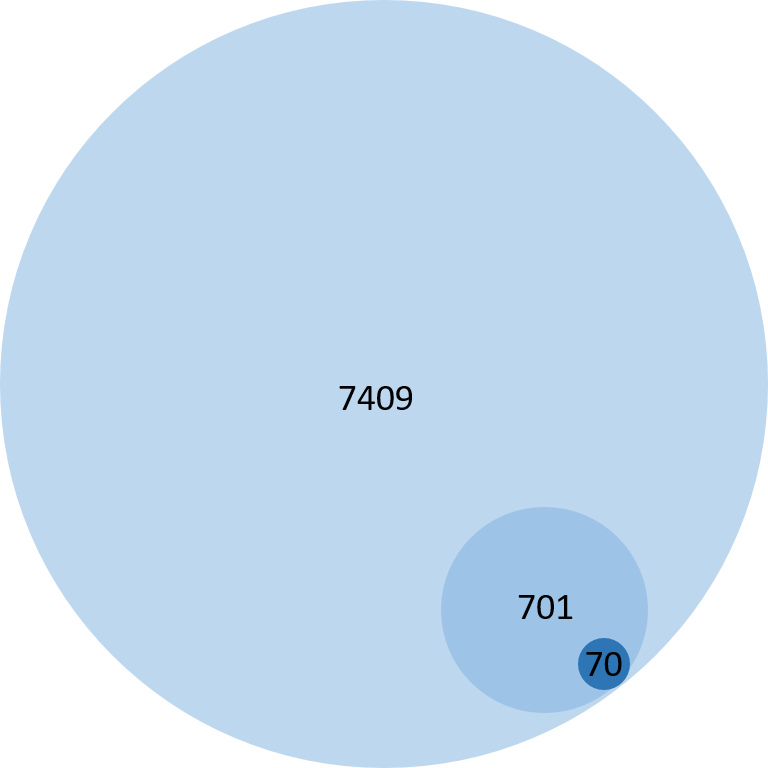
\includegraphics[height=7cm]{figures/config_var}
	\caption[Diagramm der Konfigurationsvariablen im Projekt]{Diagramm der Konfigurationsvariablen im Projekt. 70 der 701 relevanten Konfigurationsvariablen entsprechen einem Biosignalparameter, welches einem \ac{fhir}-Profil zugeordnet wurde. 
	}
	\label{fig:conf_var}
\end{figure}